\begin{figure}[H]
	\centering
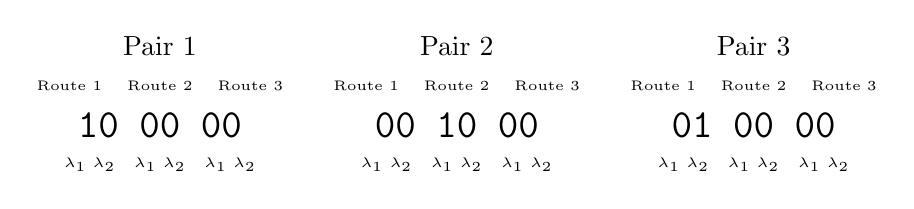
\begin{tikzpicture}[ every node/.style={align=center}]
    % First tuple
    \node at (0,1) {Pair 1};
    \node at (0,0.5) {\tiny Route 1 \quad Route 2 \quad Route 3};
    \node at (0,0) {\Large \texttt{10 00 00}};
    \node at (0,-0.5) {\tiny $\lambda_1 \ \lambda_2 \quad \lambda_1 \ \lambda_2 \quad \lambda_1 \ \lambda_2$};

    % Second tuple
    \node at (3.77,1) {Pair 2};
    \node at (3.77,0.5) {\tiny Route 1 \quad Route 2 \quad Route 3};
    \node at (3.77,0) {\Large \texttt{00 10 00}};
    \node at (3.77,-0.5) {\tiny $\lambda_1 \ \lambda_2 \quad \lambda_1 \ \lambda_2 \quad \lambda_1 \ \lambda_2$};

    % Third tuple
    \node at (7.54,1) {Pair 3};
    \node at (7.54,0.5) {\tiny Route 1 \quad Route 2 \quad Route 3};
    \node at (7.54,0) {\Large \texttt{01 00 00}};
    \node at (7.54,-0.5) {\tiny $\lambda_1 \ \lambda_2 \quad \lambda_1 \ \lambda_2 \quad \lambda_1 \ \lambda_2$};
\end{tikzpicture}
\caption{The bitstring representing a valid solution for an RWA instance where ${P} = 3, N = 3, {\Lambda} = 2$.
	%The bitstring is divided into three sub-bitstrings; each has $3 \times 2$ bits.
	%Each bit represent a selection of unique lightpath the corresponding source-destination pair.
}
\label{fig:bitstring}
\end{figure}
